%%
% The BIThesis Template for Bachelor Graduation Thesis
%
% 北京理工大学毕业设计(论文)第一章节 —— 使用 XeLaTeX 编译
%
% Copyright 2020-2021 BITNP
%
% This work may be distributed and/or modified under the
% conditions of the LaTeX Project Public License, either version 1.3
% of this license or (at your option) any later version.
% The latest version of this license is in
%   http://www.latex-project.org/lppl.txt
% and version 1.3 or later is part of all distributions of LaTeX
% version 2005/12/01 or later.
%
% This work has the LPPL maintenance status `maintained'.
%
% The Current Maintainer of this work is Huang Chenrui.
%
% 第一章节 2022/05/10

\chapter{绪论} % 引出要研究的是DQN,这是重点

\section{研究背景与意义} % 主要讲深度强化学习好,所以我们要研究它。

自动驾驶系统的决策模块需要先进的决策算法保证安全性、智能性、有效性。目前传统算法的解决思路是以价格昂贵的激光雷达作为主要传感器,依靠人工设计的算法从复杂环境中提取关键信息, 根据这些信息进行决策和判断。该算法缺乏一定的泛化能力,不具备应有的智能性和通用性。深度强化学习的出现有效地改善了传统算法泛化性不足的问题, 这给智能驾驶领域带来新的思路。

强化学习(Reinforcement Learning, RL)通过与环境交互,学习状态到行为的映射关系。如图\ref{强化学习原理}所示,在一个离散时间序列$t=0,1,2,… $中,智能体需要完成某项任务。在每一个时间$t$,智能体都能从环境中接受一个状态$S_t$,并通过动作$a_t$与环境继续交互,环境会产生新的状态$S_{t+1}$,同时给出一个立即回报$r_{t+1}$。如此循环下去,智能体与环境不断地交互,从而产生更多数据(状态和回报),并利用新的数据进一步改善自身的行为。

\begin{figure}[htbp]
  \vspace{13pt} % 调整图片与上文的垂直距离
  \centering
  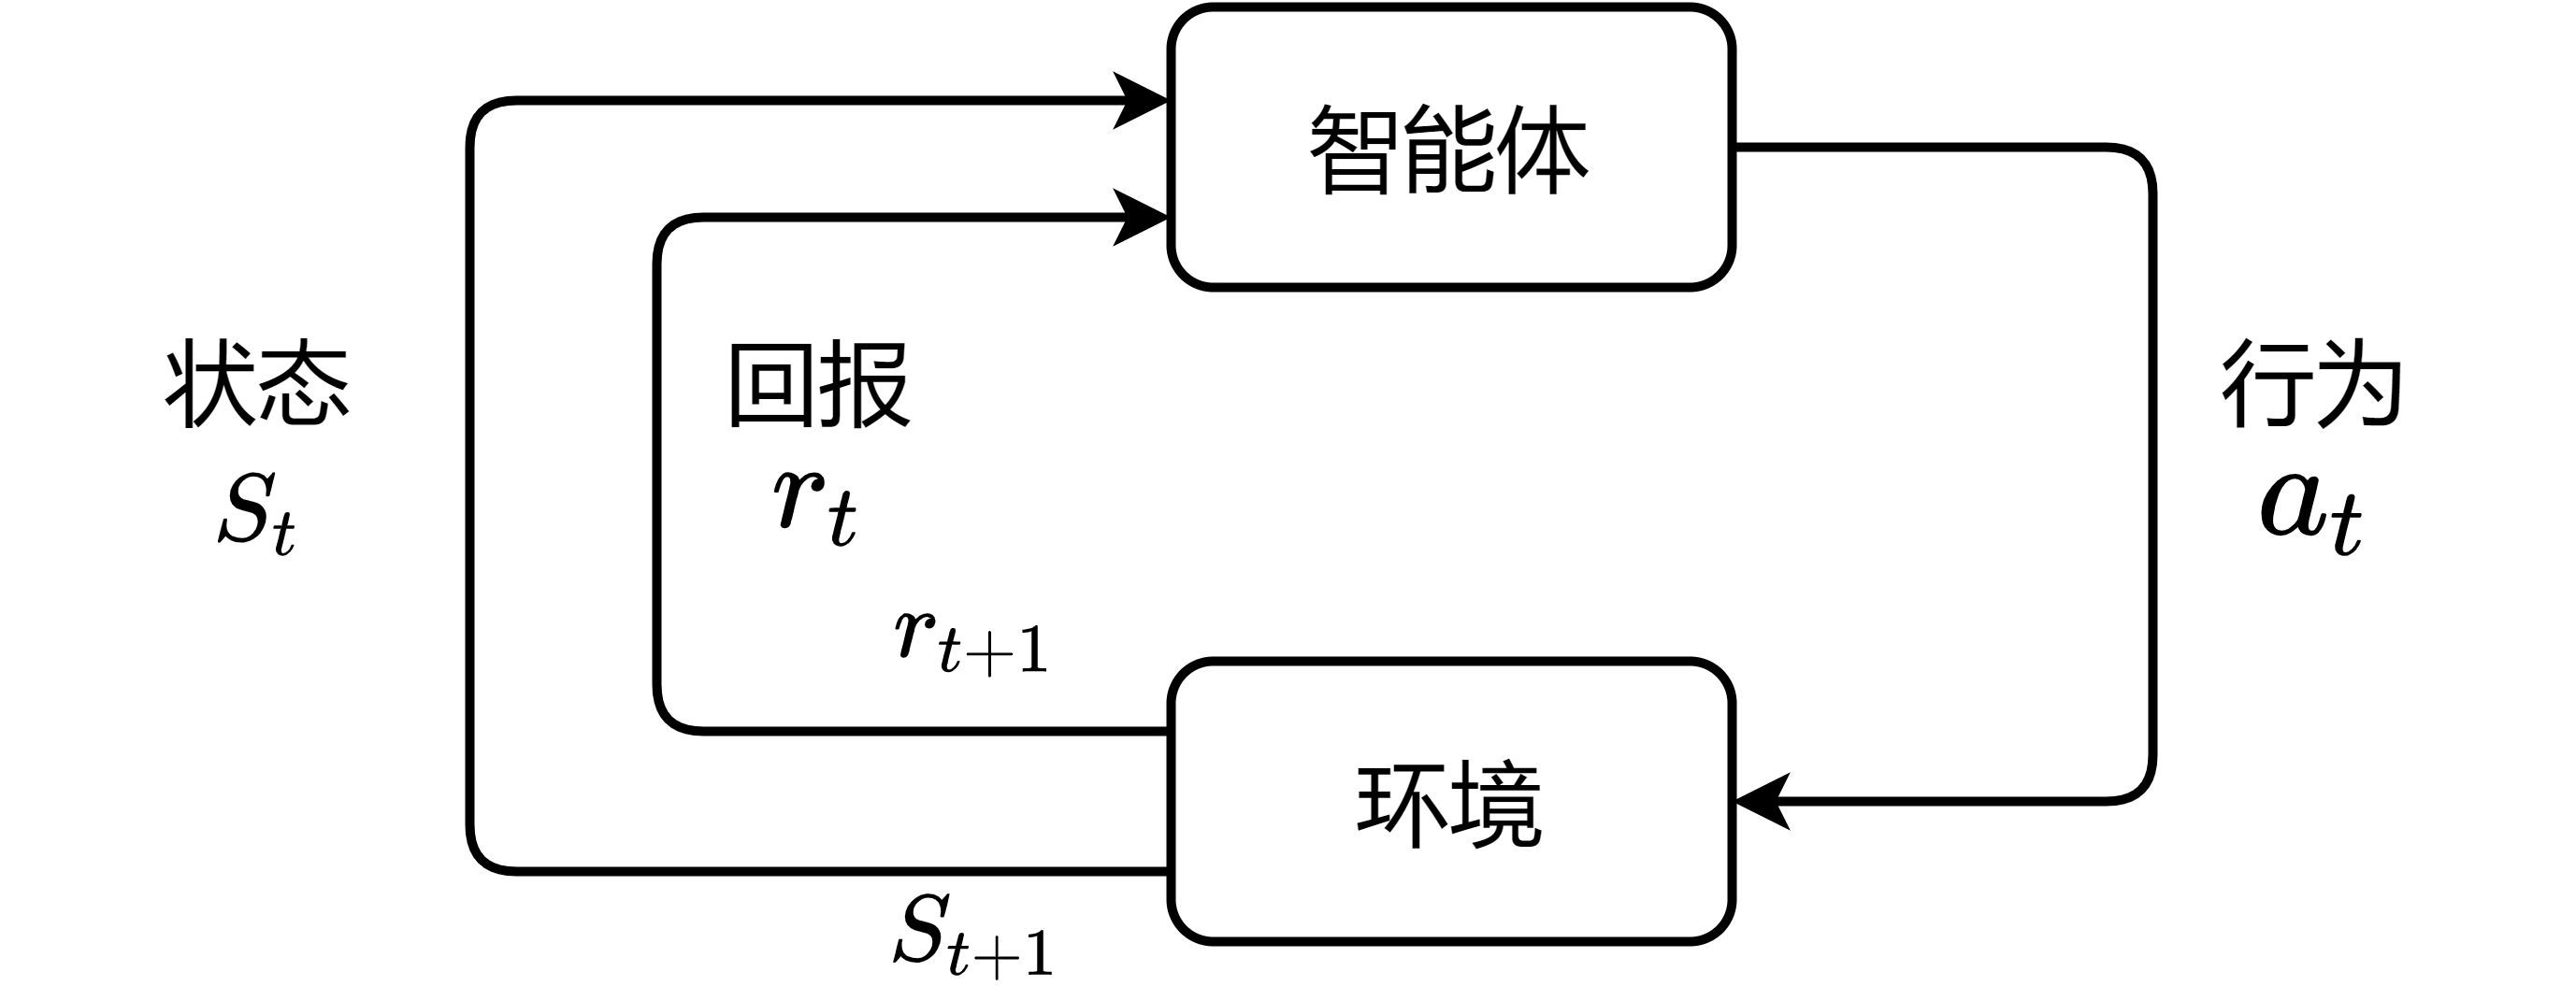
\includegraphics[width=0.73\textwidth]{images/chapter1/RL_structure.png}
  \caption{强化学习原理}\label{强化学习原理} % label 用来在文中索引
\end{figure}

目前,强化学习在策略选择的理论和算法方面已经取得了很大的进步,然而直接从高维感知输入(如图像、语音等)中提取特征,学习最优策略,对强化学习来说依然是一个挑战。

深度强化学习(Deep Reinforcement Learning, DRL)结合了深度神经网络和强化学习的优势, 可以用于解决智能体在复杂高维状态空间中的感知决策问题\cite{唐振韬2017深度强化学习进展}\cite{2017Deep}。2016年,基于深度强化学习和蒙特卡洛树搜索的AlphaGo击败了人类顶尖职业棋手,引起了全世界的关注\cite{2017Review}。 2017年, DeepMind在《Nature》上公布了最新版AlphaGo论文, 介绍了更强的围棋人工智能: AlphaGo Zero。它不需要人类专家知识, 只使用纯粹的深度强化学习技术和蒙特卡罗树搜索, 经过3天自我对弈就以100比0击败了上一版本的AlphaGo。AlphaGo Zero证明了深度强化学习的强大能力, 也必将推动以深度强化学习为代表的人工智能领域的进一步发展。基于深度强化学习在棋局与游戏上的成功,最近的研究大多注重于深度强化学习在各个领域中的扩展与应用。

综上所述,深度强化学习方法与深度神经网络强大的特征提取能力相结合,可以实现端到端的控制与决策,具有较强的通用性。通过网络自主学习的方式,减少了对系统动力学建模与数学解析的复杂度,相比于传统依据规则的决策方式更加便捷。随着人工智能的兴起和强化学习在轮式机器人相关领域的成功应用,基于深度强化学习的自动驾驶决策与控制方法为自动驾驶决策提供了新的解决方案,这使得对其研究更具有理论指导意义和实际应用价值。

\section{国内外研究现状} % 先讲端到端,再讲国内外应用,最后回归到DQN是怎么做的(DQN是本篇论文的关键点)。

自动驾驶系统(Automated driving systems, ADS)保证了安全、舒适和高效的驾驶体验,但近年来的研究表明,除非进一步提高最新技术的鲁棒性,否则自动驾驶系统的潜力便无法完全发挥\cite{2019AutoDrive}。目前,大多数的自动驾驶系统将大量的自动驾驶任务划分为若干个子类别,并在各个模块上采用一系列传感器和算法,算法流程如图\ref{模块化方法流程图}所示。

\begin{figure}[htbp]
  \vspace{13pt} % 调整图片与上文的垂直距离
  \centering
  \includegraphics[width=1.0\textwidth]{images/chapter1/Autodrive_structure.png}
  \caption{模块化方法流程图}\label{模块化方法流程图} % label 用来在文中索引
\end{figure}

最近,端到端方法开始作为模块化方法的替代出现。端到端驾驶(End-to-end driving)又被称作直接感知(direct perception)\cite{2015DeepDriving},即直接从感知输入产生动作,其算法流程图如图\ref{端到端方法流程图}所示。此处的动作可以是方向盘和踏板的连续操作,也可以是一组离散的动作,例如加速和转向。目前有三种主要的端到端方法:直接监督深度学习\cite{1989Alvinn}\cite{2016End}、神经进化\cite{1996Evolution}(neuroevolution)和最近的深度强化学习\cite{2017DRL_end_to_end}。

\begin{figure}[htbp]
  \vspace{13pt} % 调整图片与上文的垂直距离
  \centering
  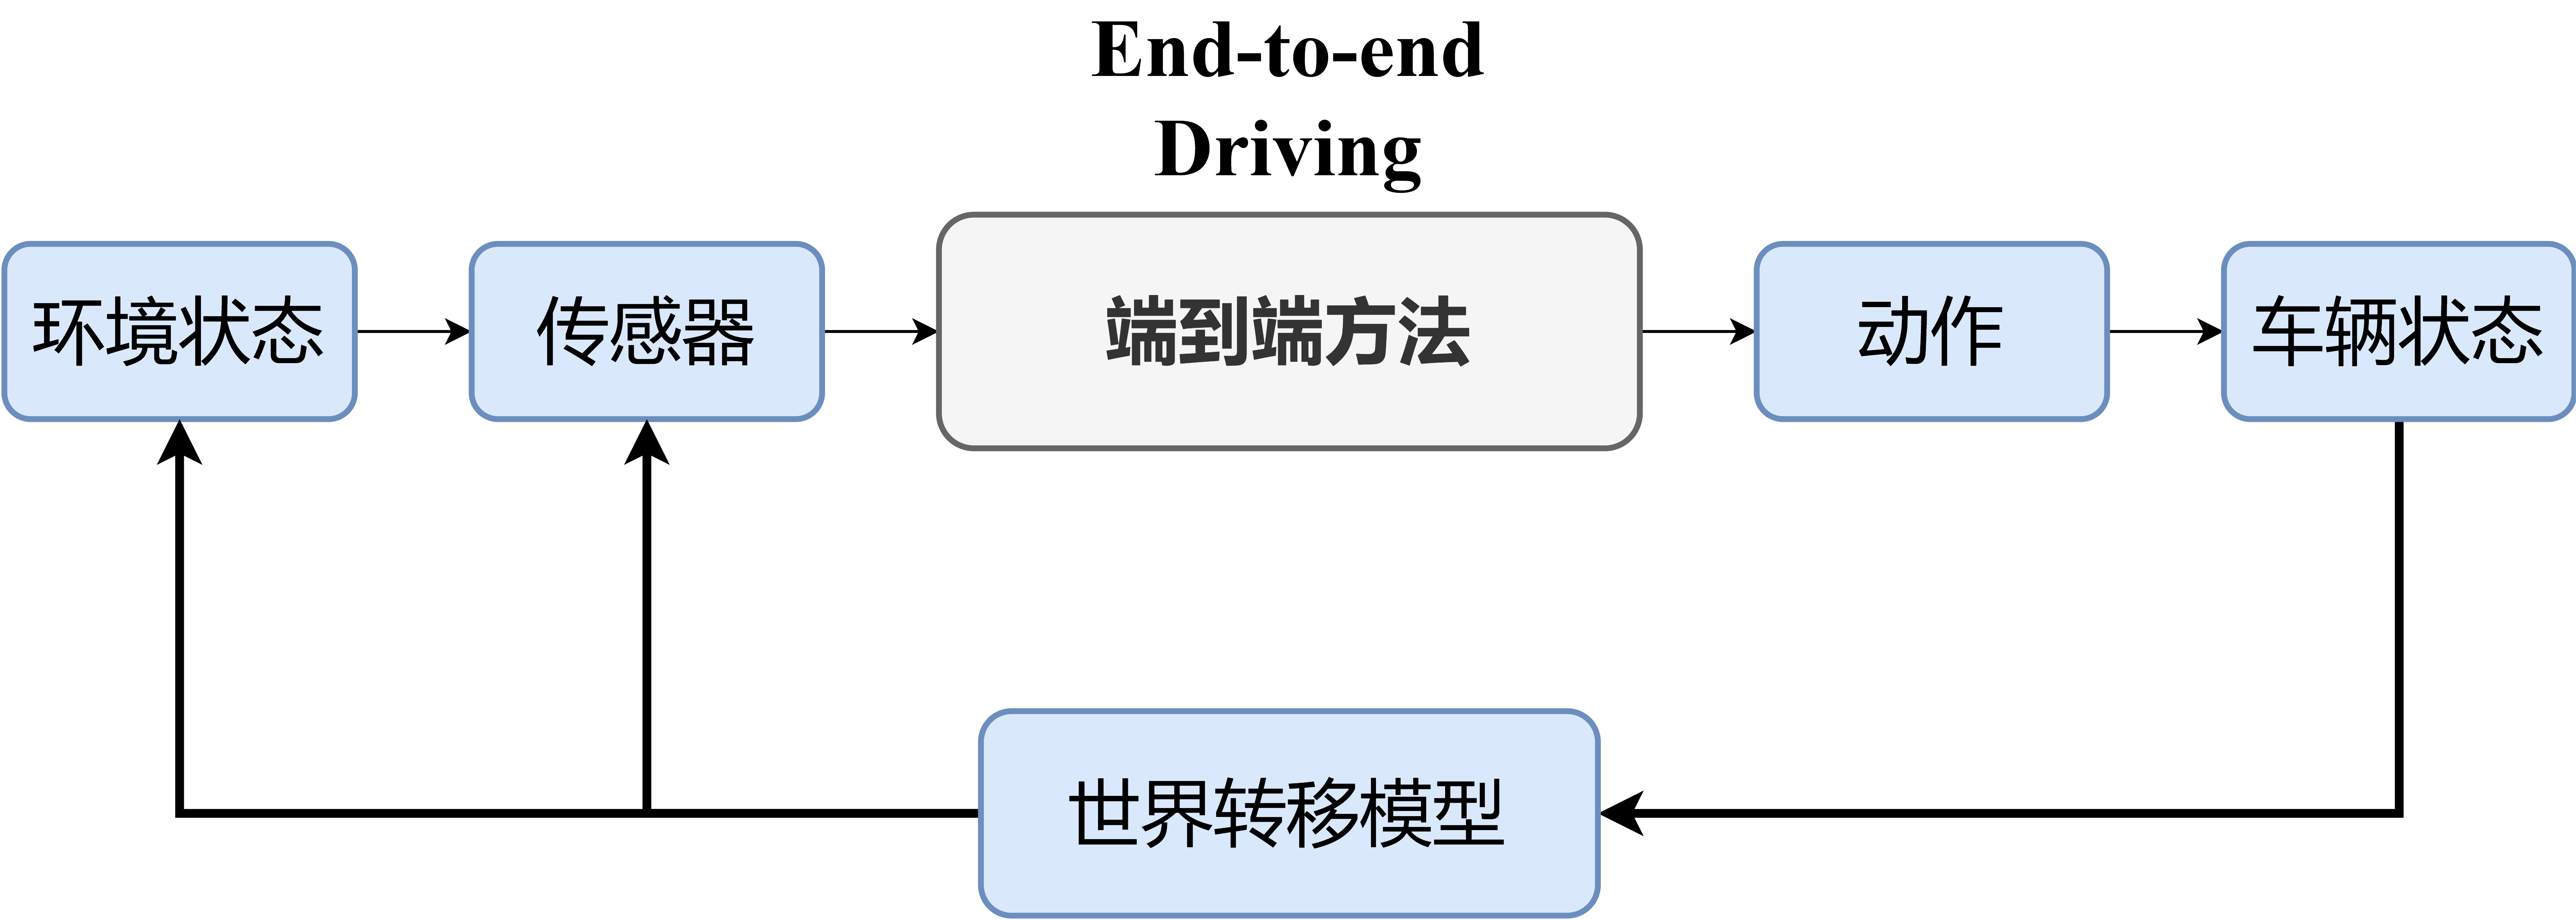
\includegraphics[width=1.0\textwidth]{images/chapter1/EndtoEnd_structure.png}
  \caption{端到端方法流程图}\label{端到端方法流程图} % label 用来在文中索引
\end{figure}

深度学习和强化学习的发展使得直接从原始的数据中提取高水平特征进行感知决策变成可能。深度学习起源于人工神经网络。早期研究人员提出了多层感知机的概念, 并且使用反向传播算法优化多层神经网络, 但是由于受到硬件等资源的限制, 神经网络的研究一直没有取得突破性进展。最近几年, 随着计算资源的性能提升和相应算法的发展, 深度学习在人工智能领域取得了一系列重大突破, 包括图像识别、语音识别、自然语言处理等。深度学习由于其强大的表征能力和泛化性能受到众多研究人员的关注, 相关技术在学术界和工业界都得到了广泛的研究与应用。

深度强化学习由数据驱动,不需要构造系统模型,具有很强的自适应能力。普林斯顿大学的Chen等使用深度学习算法, 根据摄像头采集的图像数据预测目标的距离, 同时输出操作指令\cite{2015DeepDriving}。斯坦福大学的Zhu等使用暹罗网络结构, 同时输入当前视角图像和目标物体图像, 并且使用残差网络模型提取特征. 通过A3C算法进行训练, 成功控制小车在虚拟场景和现实场景中到达指定地点\cite{2016Target}。国内的Zhao等使用深度强化学习算法和注意力机制, 实现了智能驾驶领域车辆的高精度分类\cite{2017Deepzhao}。Zhu基于TORCS的真实物理变量, 使用高斯过程强化学习算法PILCO(Probabilistic Inference for Learning Control)离线训练控制器, 实现车道保持。同时以图像为输入, 使用深度学习算法感知环境信息, 预测本车距离车到中央线距离、偏航角、道路曲率等。最终将RL的控制策略和DL的特征预测结合, 实现基于图像的车道保持。

以上研究仅由大量的数据驱动而未单独考虑模型的影响,针对自动驾驶避障技术的模型问题,德克萨斯大学奥斯汀分校的Chen等提出《Learning to drive from a world on rails》的假设\cite{2021Learning},采用世界模型与车辆模型解耦的方式建立一个前向模型来帮助改进策略;David Ha等提出生成循环神经网络以无监督的方式快速训练,通过压缩时空表征来模拟流行的强化学习环境\cite{2018Recurrent}。

%主要讲讲DQN
针对具体的深度强化学习算法,2012年,Lange等人最早在插槽赛车上使用深度强化学习算法并取得了良好的控制效果\cite{2012Autonomous}。2013年,由DeepMind团队提出的DQN(Deep Q-Network)算法利用深度卷积神经网络直接学习Atari2600种游戏的高维度图像,从输入中提取环境的高效描述,来近似最优动作-状态函数,从而习得成功策略\cite{2013DQN}。2015年,Hasselt等人发现传统的Q-learning和DQN方法都会普遍过高估计行为值函数Q值,存在过优化的问题,为了解决值函数过估计的问题,Hasselt提出了Double DQN方法,将行为选择和行为评估采用不同的值函数实现,降低了过估计的误差\cite{2015DDQN}。2016年,Ziyu Wang提出Dueling DQN方法,把Q网络的结构显式地约束成跟动作无关的状态值函数$V(s)$与在状态$s$下各个动作的优势函数$A(s,a)$之和,使得DQN训练更容易,收敛速度更快,避免因为Q值的量级大而引起的结果不稳定问题\cite{2016DuelingDQN}。2017年,Zong等人使用深度确定性策略梯度DDPG算法对智能体的加速度和转向控制进行训练,以实现自主避障,并在开源赛车模拟器(TORCS)环境中进行了测试,结果表明通过一段时间自主学习,无人驾驶汽车能学会复杂的避障换道行为\cite{2017Obstacle}。该算法是将DQN和Actor-Critic算法相结合,使用深度神经网络来逼近值函数和策略函数,虽然,DDPG算法实现了连续状态、动作空间下的强化学习,然而算法参数并不易确定,其超参数往往必须针对不同的问题进行仔细设置才能获得良好的训练结果。

随着研究的不断深入,深度强化学习算法在自动驾驶控制策略的应用范围越来越广,解决的问题也越来越复杂。这充分说明了深度强化学习算法应用于自动驾驶决策控制领域的可行性和有效性。本文在调研和分析大量文献的基础上基于深度强化学习算法设计自动驾驶决策控制算法,通过对比多种深度强化学习算法及其改进算法,验证在抽象环境与高维环境下深度强化学习算法的有效性和准确度。

\section{本文主要研究内容及章节安排} % 绪论、算法概览、两个仿真环境和改进的算法设计、结果、总结。

本文以DQN算法作为基础,探究DQN及其改进算法Double DQN和Dueling DQN在两种不同仿真环境(Highway-Env、Metadrive)中对自动驾驶决策及控制产生的效果。通过在仿真环境下的反复训练和学习,训练的模型在多种仿真环境下均具有较好的鲁棒性,证明了DQN及其改进算法在自动驾驶决策及控制方面的有效性和可行性。

第 1 章绪论。介绍了该课题的研究背景和意义,对强化学习在自动驾驶决策方面的发展现状进行了介绍,对深度强化学习特别是DQN算法的研究现状进行了详细的分析说明,在章节的最后通过分析总结参考文献得出了本文的研究方向和研究内容。

第 2 章强化学习相关算法理论分析。通过对强化学习算法原理的分析,引出了适用于无模型的 Q-learning 算法和 DQN 算法,同时,针对于DQN算法的不足和缺陷,介绍了Double DQN算法和Dueling DQN算法的原理,并对几种算法的适用场景进行了分析。

第 3 章基于DQN算法的自动驾驶避障算法设计。通过对两种仿真环境(Highway-Env、Metadrive)的分析和对比,介绍二者的状态值、动作值与奖励算法的详细情况。将DQN及其改进算法作用于两种仿真环境,同时改进Q网络的网络结构及超参数,使其完成自动驾驶决策和控制两方面的任务要求。

第 4 章实验验证。为了验证算法的可行性和有效性,进行了两种仿真环境中的仿真实验,并对具体的实验内容进行了分析与设计,对最后的实验结果进行了详细的分析与改进。

文章的最后进行了总结,对本文完成的主要工作和取得的主要成就进行了概述,对本文的创新点进行了阐述,同时指出了本文研究的不足和后续研究的重点内容。

